\documentclass[11pt,a4paper]{article}
\usepackage[utf8]{inputenc}
\usepackage{amsmath}
\usepackage{amsfonts}
\usepackage{amssymb}
\usepackage{amsthm}
\usepackage{tikz}
\usepackage{graphicx}

\usepackage{algorithm}
\usepackage{algorithmic}
\usepackage{tabularx}
\usepackage{subcaption}

\usepackage[left=2cm,right=2cm,top=2cm,bottom=2cm]{geometry}

\usepackage[resetlabels,labeled]{multibib}

\newcites{Comp}{Computation Graphs Bibliography}
\newcites{Gnn}{GNN Bibliography}

\author{Paul LANDRIER \\ Supervised by Silviu Maniu}
\title{Internship Report}

\newcommand{\bb}[1]{\mathbb{#1}}
\newcommand{\mcal}[1]{\mathcal{#1}}
\newcommand{\N}{\bb{N}}
\newcommand{\R}{\bb{R}}
\newcommand{\Cinf}{\mcal{C}^\infty}
\newcommand{\Ns}{near-semiring}
\newcommand{\sns}{sub-near-semiring}
\newcommand{\ovund}[3]{\overset{#1}{\underset{#2}{#3}}}

\newcommand{\cP}{\mathcal{P}}
\newcommand{\op}[1]{|| #1 ||_{op}}
\newcommand{\ninf}[1]{|| #1 ||_\infty}
\newcommand{\Sum}[2]{\overset{#2}{\underset{#1}{\sum}}}
\newcommand{\Prod}[2]{\overset{#2}{\underset{#1}{\prod}}}

\date{}

\usetikzlibrary{shapes}

\newtheorem{theorem}{Theorem}
\newtheorem{property}{Property}

\newtheorem{definition}{Definition}
\newtheorem{ns}{Near-semiring}

\theoremstyle{definition}
\newtheorem{corollary}{Corollary}[theorem]
\newtheorem{lemma}[theorem]{Lemma}

\renewcommand{\leq}{\leqslant}

\newcolumntype{C}[1]{>{\centering\arraybackslash}p{#1}}
\begin{document}

\maketitle

\tableofcontents

[TODO: Remove table of contents (it stays for now for better readability)]

\paragraph{abstract} TODO (Mention broad usage of computation graphs (compilers))

Paragraph in model is a good starting poitn

\section{Introduction}

TODO [Describe the interest of the computation]

\section{Modeling a Computation}

\subsection{Computation Graphs}

We try to abstract the notion of \textit{computation graphs}, having in mind the particular example of neural networks.

	Computation graphs are a type of graphs that represent a computation. Formally, in this work, we define a computation graph $(V,E,Fun,Op)$ as a directed acyclic graph $(V,E)$ together with a function $Fun:E \to F$ where $F$ is a set of functions $S \to S$ ($S$ is a fixed set, the same for all functions) and a function $Op:V \to Operator$ where $Operator$ is a set containing operators to aggregate several inputs in $S$. (Remark : usually in a computation graph, the functions are stored in the nodes and the edges represent a data dependency. We choose a different convention here to remain closer to provenance in graphs as defined in \citeComp{ramusat_semiring-based_2022}. For an other definition of computation graphs, see for instance \citeComp{Wang2023}.)
	
	For instance, if we want to compute the function $f(x)=e^{x^2}(x^2 + 2x + 2)$ using only the linear, "plus constant" and exponential functions, with $+$ and $\times$ operators, then we can model a possible computation with the computation graph :
	
	\begin{figure}[!h]
	\centering
	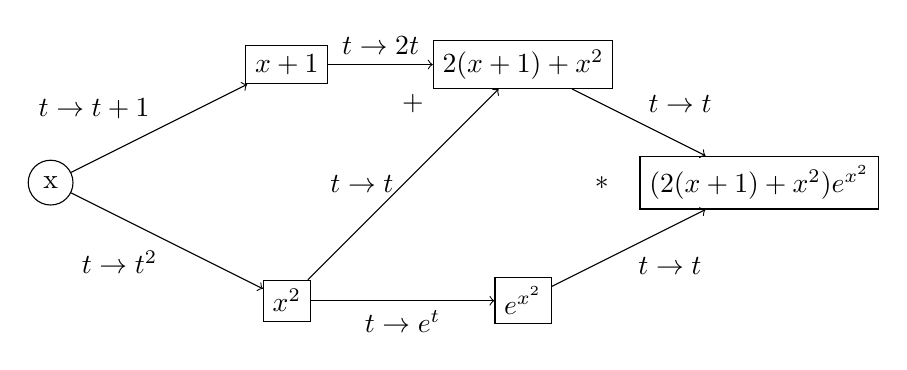
\begin{tikzpicture}
	
		\node[circle,draw] (x) at (0,0) {x};
		\node[rectangle,draw] (a) at (3,1.5) {$x+1$};
		\node[rectangle,draw] (b) at (3,-1.5) {$x^2$};
		\node[rectangle,draw] (c) at (6,1.5) {$2(x+1) + x^2$};
		\node at (4.6,1) {$+$};
		\node[rectangle,draw] (d) at (6,-1.5) {$e^{x^2}$};
		\node[rectangle,draw] (e) at (9,0) {$(2(x+1) + x^2)e^{x^2}$};
		\node at (7,0) {$*$};
		
				\path[->] (x) edge node[midway,above left] 
			{$t \to t+1$} (a);
		\path[->] (x) edge node[midway,below left]
			{$t \to t^2$} (b);
		\path[->] (a) edge node[midway,above] 
			{$t \to 2t$} (c);
			
		\path[->] (b) edge node[midway,left] 
			{$t \to t$} (c);
		\path[->] (b) edge node[midway,below] 
			{$t \to e^t$} (d);
		\path[->] (c) edge node[midway,above right]
			{$t \to t$} (e);
		\path[->] (d) edge node[midway,below right] 
			{$t \to t$} (e);
		
	\end{tikzpicture}
	\caption{One possible computation graph of $f$.}
	\label{fig:graphe_calc_ex}
	\end{figure}
	
	Let's take the example of a (non-discretized) perceptron with two inputs. If we want to model its execution using only elementary operations and the activation function $f$, we get the representation in Figure \ref{fig:perceptron}.
	
	\begin{figure}[!h]
\label{fig:graph_calc_execution}
\centering
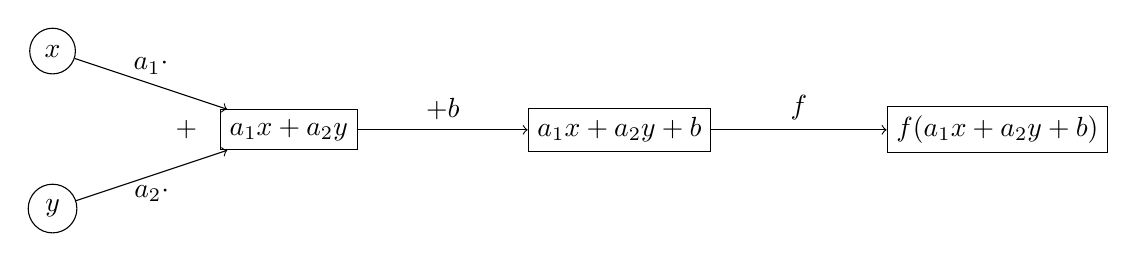
\begin{tikzpicture}

	\def\layersep{3cm}	
	
	\node[circle,draw] (x) at (0,1) {$x$};
	\node[circle,draw] (y) at (0,-1) {$y$};
	\node[rectangle,draw] (a) at (\layersep,0) {$a_1 x + a_2 y$};
	\node (plus) at (\layersep - 1.3cm,0) {+};
	\node[rectangle,draw] (c) at (2.4*\layersep,0) {$a_1 x + a_2 y + b$};
	\node[rectangle,draw] (e) at (4*\layersep,0) {$f(a_1 x + a_2 y + b)$};
	
	\path[->] (x) edge node[midway,above] {$a_1 \cdot $} (a);
	\path[->] (y) edge node[midway, below] {$a_2 \cdot$} (a);
	
	\path[->] (a) edge node[midway,above] {$ + b$} (c);
	
	\path[->] (c) edge node[midway,above] {$f$} (e);
	
	
\end{tikzpicture}
\caption{Computation graph of a perceptron.}
\label{fig:perceptron}
\end{figure}

	Since a perceptron only uses one kind of aggregation -the sum-, we shall now only consider computation graphs with one unique operator to aggregate the functions. This operator is denoted $+$ and is implicitly attached to every node in the graph.\\

In the algorithm \ref{alg:retrieve_fun}, we formalize the notion of ``function represented by a computation graph" by defining the algorithm to compute this function from the graph. We assume that there is only one node without any outgoing edge, which is the output of the computation graph, noted $out$. We also assume that we have a special function $f_v$ for each input node $v$. These special functions should be thought of as symbols, such as the ``$x$" in a definition of the form $f(x)=3x+2$.


\begin{algorithm}
\caption{Retrieving a function from a computation graph}
\label{alg:retrieve_fun}
\begin{algorithmic}[1]
\STATE \textbf{Input:} Computation Graph $G = (V, E, Fun, Op)$.
\STATE \textbf{Output:} The function represented by the graph.
\STATE
\STATE \textbf{Function} Retrieve(G):
\STATE \quad Let $T$ be a topological ordering of $(V,E)$.
\STATE \quad \textbf{Initialize:} $Function[v]$ = None for all $v \in V$
\STATE \quad \textbf{for each} $v$ in $T$ \textbf{do}
\STATE \quad \quad \textbf{if} $v$ is an input node \textbf{then}
\STATE \quad \quad \quad $Function[v]=f_v$.
\STATE \quad \quad \textbf{else}
\STATE \quad \quad \quad \textbf{Initialize:} $f=0$
\STATE \quad \quad \quad \textbf{for each} edge $e=(u,v)$ entering $v$ \textbf{do}
\STATE \quad \quad \quad \quad $f=f + (Fun(e) \circ Function[u])$
\STATE \quad \textbf{return} $Function[out]$
\end{algorithmic}
\end{algorithm}

	In the section \ref{subsec:Properties of Generalized Computation Graphs}, we prove that the result does not depend on the topological ordering chosen in the execution of the algorithm.

\subsection{Model}

[TODO: is modularity a good term ?]

	In \citeComp{green_provenance_2007} and \citeComp{ramusat_semiring-based_2022}, the authors defined a set of identities and restrictions on the object of their studies (respectively relational databases and graph databases) and then used this set to identify an algebraic structure to theoretically model them.
	
	We follow the same method to characterize the minimal algebraic structure required to model a computation graph. An example of generalized computation graph is given in Figure \ref{fig:graphe_calc_abstr}. In what follows, we describe the different properties of computation graphs and traduce them algebraically. The process is summarized in the table of Figure \ref{fig:table_algebraic_structure} and specific instances where the described properties are necessary are presented in Figure \ref{fig:drawings_algebraic_struct}. In the examples of Figure \ref{fig:drawings_algebraic_struct}, the symbolic functions are omitted for better readability.

	\begin{figure}
	\centering
	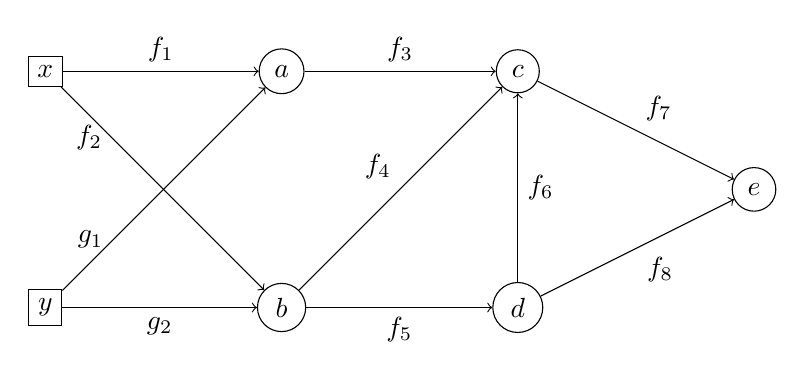
\begin{tikzpicture}
	
		\node[rectangle,draw] (x) at (0,1.5) {$x$};
		\node[rectangle,draw] (y) at (0,-1.5) {$y$};
		\node[circle,draw] (a) at (3,1.5) {$a$};
		\node[circle,draw] (b) at (3,-1.5) {$b$};
		\node[circle,draw] (c) at (6,1.5) {$c$};
		\node[circle,draw] (d) at (6,-1.5) {$d$};
		\node[circle,draw] (e) at (9,0) {$e$};
		
		\path[->] (x) edge node[midway,above] 
			{$f_1$} (a);
		\path[->] (x) edge node[near start, left=0cm]
			{$f_2$} (b);
		\path[->] (y) edge node[near start, left=0cm] 
			{$g_1$} (a);
		\path[->] (y) edge node[midway,below]
			{$g_2$} (b);
		\path[->] (a) edge node[midway,above] 
			{$f_3$} (c);
			
		\path[->] (b) edge node[midway,above left] 
			{$f_4$} (c);
		\path[->] (b) edge node[midway,below] 
			{$f_5$} (d);
		\path[->] (d) edge node [midway,right] 
			{$f_6$}(c);
		\path[->] (c) edge node[midway,above right]
			{$f_7$} (e);
		\path[->] (d) edge node[midway,below right] 
			{$f_8$} (e);
		
	\end{tikzpicture}
	\caption{A generalised computation graph.}
	\label{fig:graphe_calc_abstr}
	\end{figure}

	\paragraph{Structure needed} We consider a structure $(F,\circ,+,0,id)$. The $+$ and $\circ$ are operators $F^2 \to F$ respectively used to model aggregation and composition in the computation graph.

Firstly, since there is no natural order on incoming edges for a node, $+$ must be associative and commutative so the sum on incoming edges is well-defined. For an example, see the Figure \ref{subfig:drawings_plus}.

	We require the operator $\circ$ to be associative to ensure modularity. For an example, see the Figure \ref{subfig:drawings_comp}.

	To abstract the concept of zero-weight, we require the existence of a neutral element $0$ which is a left absorbing element for the $\circ$ operator and which is a neutral element for $+$. For an example, see the Figure \ref{subfig:drawings_zero}.

	We require the left distributivity $(f+g) \circ h = f \circ h + g \circ h$ beacuse it is of theoretical interest (it is necessary for the interpretation of near-semirings as sub-near-semirings of the the complete near-semiring over a monoid), because it is a natural identity to interpret the elements as functions and because it allows for a simplification of the computation in some cases. For an example, see the Figure \ref{subfig:drawings_distr}.

	Finally, we require the existence of a neutral element $id$ for $\circ$. This might not be crucial, but it has interesting theoretical properties -it matters for theorem \ref{thm:near_semirings_fun_monoids}- and allows some natural representation. For an example, see the Figure \ref{subfig:drawings_id}.
	\\

	\begin{figure}
		\centering
		\begin{tabular}{|C{7.5cm}|C{7.5cm}|}
			\hline 
			\textbf{Property on the computation graph} & \textbf{Algebraic traduction of the property} \\ 
			\hline 
			The edges that enter a node are not ordered & + is associative and commutative \\ 
			\hline
			The concatenation of two computation graphs is a computation graph that represent the composition of the functions & $\circ$ is associative \\ 
			\hline 
			There is a notion of zero-weight that model the fact that there is no interaction between two nodes. & There is a $0_F$ element that is a neutral element for $+$ and that is left absorbing for $\circ$. \\ 
			\hline 
			We can reuse computation previously done in a natural way. & The operator $\circ$ is right distributive over $+$. \\ 
			\hline 
			We should be able to model the identity function. & There is a neutral element $id$ for $\circ$. \\ 
			\hline 
		\end{tabular} 
	\caption{Motivation of the algebraic structure.}
	\label{fig:table_algebraic_structure}
	\end{figure}

\begin{figure}
	\centering
	\begin{subfigure}{\textwidth}
	\centering
		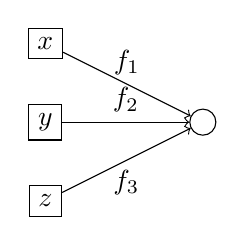
\begin{tikzpicture}
			\node[rectangle,draw] (x) at (-2.5,1) {$x$};
			\node[rectangle,draw] (y) at (-2.5,0) {$y$};
			\node[rectangle,draw] (z) at (-2.5,-1) {$z$};
			\node[circle,draw] (res) at (-0.5,0) {};
			
			\path[->,draw] (x) -- node[midway,above] {$f_1$} (res);
			\path[->,draw] (y) -- node[midway,above] {$f_2$} (res);
			\path[->,draw] (z) -- node[midway,below] {$f_3$} (res);
		\end{tikzpicture}
		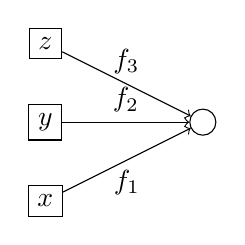
\begin{tikzpicture}
			\node[rectangle,draw] (x) at (0,-1) {$x$};
			\node[rectangle,draw] (y) at (0,0) {$y$};
			\node[rectangle,draw] (z) at (0,1) {$z$};
			\node[circle,draw] (res) at (2,0) {};
			
			\path[->,draw] (x) -- node[midway,below] {$f_1$} (res);
			\path[->,draw] (y) -- node[midway,above] {$f_2$} (res);
			\path[->,draw] (z) -- node[midway,above] {$f_3$} (res);
		\end{tikzpicture}
		\caption{A case that necessits the ``$+$" operator to be commutative and associative. Indeed, these two graphs are the same represented in two different ways, and the left one represent the element $(f_1+f_2)+f_3$ whereas the right one represents $(f_3 + f_2) + f_1$. Replacing $f_3$ by $0$ then shows that $+$ must be comutative, and using the commutativity of $+$ shows that the right expression is equal to $f_1 + (f_2 + f_3)$, so the associativity is required too.}
		\label{subfig:drawings_plus}
	\end{subfigure}

	\begin{subfigure}{\textwidth}
	\centering
		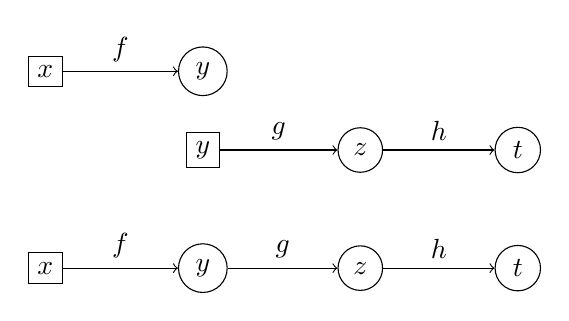
\begin{tikzpicture}
		
			\node[rectangle,draw] (x) at (0,0) {$x$};
			\node[circle,draw] (y) at (2,0) {$y$};
			\node[rectangle,draw] (y') at (2,-1) {$y$};
			\node[circle,draw] (z') at (4,-1) {$z$};
			\node[circle,draw] (t') at (6,-1) {$t$};
			
			\node[rectangle,draw] (xf) at (0,-2.5) {$x$};
			\node[circle,draw] (yf) at (2,-2.5) {$y$};
			\node[circle,draw] (zf) at (4,-2.5) {$z$};
			\node[circle,draw] (tf) at (6,-2.5) {$t$};
			
			\path[->,draw] (x) -- node[midway,above] {$f$} (y);
			\path[->,draw] (y') -- node[midway,above] {$g$} (z');
			\path[->,draw] (z') -- node[midway,above] {$h$} (t');
			
			\path[->,draw] (xf) -- node[midway,above] {$f$} (yf);
			\path[->,draw] (yf) -- node[midway,above] {$g$} (zf);
			\path[->,draw] (zf) -- node[midway,above] {$h$} (tf);
		
		\end{tikzpicture}	
		\caption{Necessity of the associativity for the modularity. The fact that the graph below, which associated element is $h\circ (g \circ f)$, represents the same element as the composition of the two graphs above, which associated element is $(h \circ g) \circ f$, is equivalent to the associativity of $\circ$. Then we can say without ambiguity that they both represent $h \circ g \circ f$.}
		\label{subfig:drawings_comp}
	\end{subfigure}

	\begin{subfigure}{\textwidth}
		\centering
		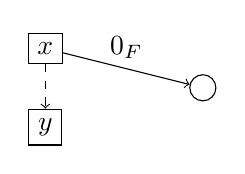
\begin{tikzpicture}
			\node[rectangle,draw] (x) at (0,0.5) {$x$};
			\node[rectangle,draw] (y) at (0,-0.5) {$y$};
			\node[circle,draw] (res) at (2,0) {};
			
			\path[->,draw] (x) -- node[midway,above] {$0_F$} (res);
			\path[->,dashed,draw] (x) -- (y);
		\end{tikzpicture}	
		\caption{Use-cases of the 0 weight. The plain arrow represent an existing edge with weight 0 (in the context of neural network for instance) and the dashed arrow represent an edge that does not exist and could be represented by the 0 element, which could for instance be used to model computation graphs as adjacency matrices.}
		\label{subfig:drawings_zero}
	\end{subfigure}

	\begin{subfigure}{\textwidth}
		\centering
		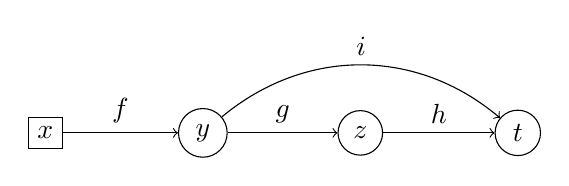
\begin{tikzpicture}
			\node[rectangle,draw] (x) at (0,0) {$x$};
			\node[circle,draw] (y) at (2,0) {$y$};
			\node[circle,draw] (z) at (4,0) {$z$};
			\node[circle,draw] (t) at (6,0) {$t$};

			\path[->,draw] (x) -- node[midway,above] {$f$} (y);
			\path[->,draw] (y) -- node[midway,above] {$g$} (z);
			\path[->,draw] (z) -- node[midway,above] {$h$} (t);
			\path[->,draw] (y) edge [bend left=40] node[midway,above] {$i$} (t);
		\end{tikzpicture}
		\caption{Illustration of the modularity allowed by the right distributivity. We can factor the expression $i~\circ~f+h~\circ~g~\circ~f$ in the smaller one $(i + g \circ h) \circ f$.}
		\label{subfig:drawings_distr}
	\end{subfigure}

	\begin{subfigure}{\textwidth}
		\centering
		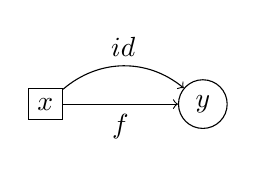
\begin{tikzpicture}
			\node[rectangle,draw] (x) at (0,0) {$x$};
			\node[circle,draw] (y) at (2,0) {$y$};
			
			\path[->,draw] (x) -- node[midway,below] {$f$} (y);
			\path[->,draw] (x) edge [bend left=40] node[midway,above] {$id$} (y);
		\end{tikzpicture}
		\caption{A use case of the identity: representing $f(x) + x$.}
		\label{subfig:drawings_id}
	\end{subfigure}
\caption{The situations that justify the different properties discussed in Figure \ref{fig:table_algebraic_structure}.}
\label{fig:drawings_algebraic_struct}
\end{figure}

The axiom identified are those of a near-semiring, with two differences (+ is not assumed to be commutative in general and the ``id" does not necessarily exist). In our case, we obtain the definition:

\begin{definition}[Near-semiring]

	A \textit{near-semiring} $(F,+,\circ,0_F,id)$ is a set $F$ equiped with two binary operations $+,\circ$ and two distinguished elements $0_F,id$ such that :
	
	\begin{itemize}

		\item $(F,+,0_F)$ is a commutative monoid;

		\item $(F,\circ,id)$ is a monoid;

		\item $\forall (f,g,h) \in F^3$, $(f+g) \circ h = f \circ h + g \circ h$;

		\item $0_F$ is left absorbing for $\circ$, i.e. for all $f \in F$, $0_F \circ f = 0_F$.

	\end{itemize}

\end{definition}

Together with this definition comes the notion of morphism of near-semiring and of sub-near-semiring:

A sub-near-semiring of a near-semiring $(F,+,\circ,0,id)$ is a subset $G \subset F$ such that $0 \in G, id \in G$ and $G$ is stable by $+$ and $\circ$. If $G$ is a sub-near-semiring of $(F,+,\circ,0,id)$, then $(G,+,\circ,0,id)$ (for the restriction of operations + and $\circ$ to $G$) forms a near-semiring.

If $(F,+,\circ,0,id)$ and $(G,+',\circ ',0',id')$ are two near-semirings, then $\phi : F \to G$ is said to be a near-semiring morphism if it satisfies $\phi(0)=0',\phi(id)=id',\forall (f,g) \in F^2, \phi(f+g) = \phi(f) +' \phi(g)$ and $ \phi(f \circ g)= \phi(f) \circ' \phi(g)$. The image $\phi(F)$ is a sub-near-semiring of $G$.



\subsection{Examples of Near-semirings}

Before establishing further theoretical results, we give a few examples of near-semirings. 

\begin{ns}[Complete near-semiring over a monoid]
\label{ns:ns_over_a_monoid}
	Let $(M,+,0_M)$ be a monoid. We define $\mcal{F}$ the set of all functions $M \to M$. Then $(\mcal{F},+,\circ,0_F,id)$ where $0_F : x \mapsto 0_M$ is the zero function and $id : x \mapsto x$ is the identity function is a near-semiring, that we will call complete \Ns\ over $M$. A particular sub-\Ns\ of $\mcal{F}$ is the set of monoid endomorphisms of $M$ (it is even a semiring). As we shall see later in this work, this is the most general kind of near-semiring in some sense.
\end{ns}

\begin{ns}[]

The $\mathcal{C}^\infty$ functions over the real numbers form a near-semiring with usual addition, composition, zero function and identity.

\end{ns}

\begin{ns}[Semirings]
\label{ns:semirings}
	Let $(S,+,\cdot,0,1)$ be a semiring. Then $(S,+,\cdot,0,1)$ is also a \Ns . Indeed, the axioms of \Ns\ are stricly more general than those of a semiring. The interpretation of semirings as sets of function together with the interpretation of $\cdot$ as a composition can be made through the structure of semimodules, which is itself a sub-\Ns\ of the complete \Ns\ over a monoid.
\end{ns}

\subsection{Properties of Generalized Computation Graphs}
\label{subsec:Properties of Generalized Computation Graphs}

We now provide two theoretical properties on computation graphs. These two properties ensure that the model 

\begin{property}
	The output of algorithm \ref{alg:retrieve_fun} does not depend on the topological ordering chosen in the execution.
\end{property}

\begin{proof}

	We consider a computation graph $G = (V,E,Fun,Op)$ and two topological orderings $T_1 ,T_2$. We note $n = |V|$. We use the notations of algorithm \ref{alg:retrieve_fun} with an index 1 or 2 to refer to the execution that is considered.
	
	 We proceed by induction on $i \in [|0,n|]$ with the hypothesis $H_i$: ''For all $1 \leq k \leq i$, if we note $v_k$ the $k$-th node according to the ordering $T_1$, then $Function_1[v_k]=Function_2[v_k]$".
	 
	 In the base case, $i=0$ and there is nothing to prove. We now consider $i \in [|0,n|]$, assume $H_i$ is verified and prove that $H_{i+1}$ is verified as well.
	 
	 We only need to prove that $Function_1[v_{i+1}]=Function_2[v_{i+1}]$.\\
	 
	 If $v_{i+1}$ is an input node, then $Function_1[v_{i+1}]=f_{v_{i+1}}=Function_2[v_{i+1}]$.
	 
	 Else, by definition, $Function_1[v_{i+1}]=\Sum{e=(u,v_{i+1}) \in E}{} Fun(e) \circ Function_1[u]$. However, since all the vertices $u$ that appear in the sum are before $v$ in the topologicale ordering, by the induction hypothesis this can be rewritten: $Function_1[v_{i+1}]=\Sum{e=(u,v_{i+1}) \in E}{} Fun(e) \circ Function_2[u]=Function_2[v_{i+1}]$, which conclude the proof.
\end{proof}

Note that the only thing required by the proof is that the result of the aggregation operation $+$ (denoted by $\sum$ in the computation) does not depend on the order of its arguments.\\

\begin{property}[Modularity of computation graphs]
	We consider two computation graphs $G_1,G_2$ over the same near-semiring $(F,+,\cdot,0,id)$. We asuume that $G_1$ has only one output node and that $G_2$ has only one input node. 
	
	We define $G_{1 \circ 2}$ as the computation graph that contains the disjoint union of $G_1$ and $G_2$ with one edge with weight $id$ that connects the output of $G_1$ to the input of $G_2$. We assume that the symbolic function associated to the input of $G_2$ is $id$.
	
	Then we have $Retrieve(G_{1 \circ 2}) = Retrieve(G_2) \circ Retrieve(G_1)$.
\end{property}

	The assumption done on the symbolic function of the only input of $G_2$ is natural: the symbolic functions are required to distinguish between the inputs, when there is only one input it is not necessary to use them.
	
	[TODO: interpretation of graphs as black boxes]
	
\begin{proof}
12
\end{proof}


\subsection{Universal Object}

TODO write this properly:

In Ramusat we had :
	The full computation represented by the graph cannot be expressed in a similar fashion as for provenance in graphs ($\underset{\pi \in P_{x,y}}{\sum} w(\pi)$) because composition does not distribute over $+$.
In Green : polynomials

Us ?
\\


Given a \Ns\ $F$, we want to characterize the sub-near-semiring generated by a subset $G \subset F$. This notion makes sense for the usual reason: an intersection of sub-near-semiring is a \sns\ itself, and we note $<G>$ this \sns\ .

For this purpose we define a sequence of sets $(G_n)$ by $G_0=\{0,id\} \cup G$ and 
$$G_{n+1} = \left\{ \left. g \circ \left( \overset{k}{\underset{i=1}{\sum}} g_i \right) \right| \ k \in \N, g \in G, (g_i)_{1 \leq i \leq n} \in (G_n)^k \right\} .$$

	The claim is now that $<G> = \underset{n \in \N}{\cup} G_n$. Indeed, $G \subset G_0 \subset \underset{n \in \N}{\cup} G_n$, then we show by induction that $\forall n \in \N, G_n \subset <G>$ and finally we show that $\underset{n \in \N}{\cup} G_n$ is indeed a \sns\ of $F$.
	
	[TODO: Write this proof cleanly or rewrite the section]

\subsection{Generality of the Complete Near-semiring over a Monoid.}

\begin{theorem}{Universal Form of Near-semirings}
\label{thm:near_semirings_fun_monoids}

	It is equivalent to be given:

	\begin{enumerate}

		\item a near-semiring $(F,+,\circ,0,id)$

		\item a commutative monoid $(M,+,0)$ together with a set of functions $M \to M$ containing $0$ and $id$ and stable by $\circ$ and $+$. (I.e. a \sns\ of the complete \Ns\ over $M$.)

	\end{enumerate}

\end{theorem}

\begin{proof}

	Firstly, we assume that we are given a monoid $(M,+,0)$ and a set of functions $M \to M$ containing $0$, $id$ and stable by $+$ and $\circ$ like in two. This precisely means that we are given a sub-near-semiring of the complete near-semiring over $(M,+,0)$, and hence a near-semiring.
	
	Secondly, if we are given a near-semiring $(F,+,\circ,0,id)$, we define for an element $f$ the function 
	$$\bar{f} : \left\{ 
	\begin{array}{c c c}
		F & \to & F \\
		g & \mapsto & f \circ g
	\end{array} \right. ,$$
	then we define the function $\phi : \left\{ 
	\begin{array}{c c c}
		F & \to & ((F,+,0) \to (F,+,0)) \\
		f & \mapsto & \bar{f}
	\end{array} \right.$. 
	
	The function $\phi$ is a morphism of near-semirings. Indeed: 
	\begin{itemize}
	
		\item $\phi(0)$ is the zero function since zero is left absorbing,
		
		\item $\phi(id)$ is the identity function because $\forall g \in F,id \circ g= g$,
		
		\item $\forall f_1,f_2 \in F^2,\ \forall g \in F,\ \phi(f_1 + f_2)(g)=(f_1 + f_2) \circ g = f_1 \circ g + f_2 \circ g = \phi(f_1)(g) + \phi (f_2)(g)$, hence $\phi(f_1+f_2)=\phi(f_1)+\phi(f_2)$
		
		\item $\forall f_1,f_2 \in F^2,\ \forall g \in F,\ \phi(f_1 \circ f_2)(g)=(f_1 \circ f_2) \circ g = f_1 \circ (f_2 \circ g) = \phi(f_1)(f_2 \circ g) = (\phi(f_1) \circ \phi(f_2))(g) $, hence $\phi(f_1 \circ f_2)=\phi(f_1) \circ \phi(f_2)$
	
	\end{itemize}
	Therefore, $\phi(F)$ is a sub-near-semiring of the complete near-semiring over the monoid $(F,+,0)$.

\end{proof}

	This theorem is interesting because it clearly indicates a direction for further investigation -if we want to instantiate the theoretical framework, we should define computation graphs over some monoids- and a limit of the expresiveness of the theory. However, it does not provide any information on the structure of near-semirings.


It might be interesting to note that for the example of computation graphs we restrict ourselves to finitely generated monoids, because the computation only involves a finite number of elements.

\section{Instantiation of the Theory}

	\subsection{Layer-Wise Relevance Propagation}
	
		[Founded on LRP overview, https://iphome.hhi.de/samek/pdf/MonXAI19.pdf]
		
		[Dependance or not on an execution, want to do the computation once or several times]
		
	Layer-Wise Relevance Propagation (LRP) is a technique used to explain the prediction made by a neural network on one of its execution. The idea of the technique is to propagate backwards the contribution (or the \textit{relevance}) of neurons in the network to the final prediction of the model. The general formula is 
		$$ R_j = \underset{k}{\sum} \frac{z_{j,k}}{\sum_j z_{j,k}} R_k .$$
		
	The value $R_j$ is the score of the neuron $j$, and it is computed by summing over all neurons $k$ in the next layer the term $\frac{z_{j,k}}{\sum_j z_{j,k}} R_k$, where $R_k$ is the relevance of neuron $k$ and $\frac{z_{j,k}}{\sum_j z_{j,k}}$ represents the extent to which neuron $j$ contributed to the relevance of the neuron $k$.
		
	The normalization term ensures that vanishing phenomenoms cannot occur: the sum of the relevances of neurons on a given layer is preserved.
		\\
		
	We should now discuss the interpretation of LRP as an instantiation of our model.
		
	We can model LRP with generalized computation graphs. Indeed, the input nodes of the computation graphs are the output neurons of the network (or even the only neuron corresponding to the class predicted, since the value of other neurons is set to zero), the edges of the computation graph are the reversed edges of the neuron and the associated function is the multiplication by the scalar $\frac{z_{j,k}}{\sum_j z_{j,k}}$ (between neurons $k$ and $j$).
	
		
\subsection{Quantization}
	
	[TODO: Quantization]
	
\section{Conclusion}

	[TODO]
	
	\bibliographystyleComp{apalike}
	\bibliographyComp{biblio_computation_graphs}	
	
\section{Extra work - GNN Stability}
	While investigating the possibility to theoretically model a neural network, I met a Ph.D student that was working on graph neural networks (GNN). GNNs are used to embed graphs in metric spaces and its objective is to extend this technique in order to embed databases.
	
	My contribution in this work was to adapt result on stability to our precise setting, and the hypotheses used in our work even allowed me to improve existing results.

	A graph neural network (GNN) is a particular type of neural network that is meant to represent graph-structured data in $\R^d$ while taking into account the relations between the data points. Such representations, or embeddings, are interesting because we can then apply usual machine learning techniques to the transformed data.
	
	However, for such schemes to be meaningful we need to ensure that the embeddings are coherent 

\subsection{Definition of GNNs}

	

\subsection{Formal Framework for Stability}

To measure the distance between two graph shift operators, and consequently the distance between the graphs they are derived from, we use $d_{\cP}(S, \hat{S})$, noted $||S - \hat{S}||_\cP$ in \citeGnn{gama2020stability},  defined as $d_\cP(S,\hat{S})=\underset{P \in \cP}{\min} ||S-P \hat{S} P^T ||$ where $\cP$ is the set of permutation matrices. We change the notations to highlight the fact that the quantity depends on the two matrices $S,\hat{S}$ and not on the difference $S-\hat{S}$. The definition of $d_\cP$ can be extended to general continuous operators $\Psi, \hat{\Psi}: \mathbb{R}^N \to \mathbb{R}^N$ by $d_\cP (\Psi, \hat{\Psi}) = \underset{P \in \cP}{\min} \ \underset{||x|| = 1}{\max} \ || P^T \Psi (x) - \hat{\Psi}(P^T x) ||$.

        
\paragraph{Limitations} There are two main challenges to apply the preceding framework. Firstly, computing $d_\cP(S,\hat{S})$ is more general than determining if the graphs are isomorphic, so it is not feasible for large $n$ in general. (Indeed, if $S$ is the adjacency matrix, then two graphs $G$ and $\hat{G}$ are isomorphic if and only if there exists $P \in \cP$ s.t. $S=P \hat{S} P^T$, which is equivalent to $d_\cP(S,\hat{S})=0$.) Secondly, we can only compare matrices that have the same size, i.e. graphs that have the same number of nodes. However, we seek to measure the perturbation induced by the deletion of tuples in the database, which corresponds to node deletion in the graph.

\paragraph{Solution used in this work} We consider a database $D$ with associated graph $G$. Let $T$ be a set of tuples of $D$, let $\hat{D}$ be the database $D$ without the tuples in $T$ and let $\hat{G}$ be its associated graph. We define their two graph shift operators $S$ and $\hat{S}$. There are two equivalent points of view for our approach:
      
\begin{itemize}
    \item We fill the matrix $\hat{S}$ with rows and columns of $0$s so its shape matches the shape of $S$. Then we consider the permutation $\sigma_0$ that matches the remaining nodes in $\hat{G}$ with their original node in $G$ and matches the rows/columns of $0$s with the nodes in $G$ that disappeared in $\hat{G}$. The permutation $\sigma_0$ provides us a permutation matrix $P_0$ and we bound $d_\cP(S,\hat{S})$ by $||S-P_0 \hat{S} P_0^T||_{op}$.

    \item We do not delete the nodes we are supposed to delete, but delete their edges instead. This yields a graph $\hat{G}'$ with exactly the same nodes as $G$ but some missing edges, and we compute $\op{S-\hat{S}'}$.
\end{itemize}

\subsection{Theoretical results}

    We take advantage of the fact that we only use filters that are polynomial of order 1 to refine the theorem 4 of \citeGnn{gama2020stability}. The two main improvements that are allowed by this simplification is the fact that the inequality is now a global inequality and there is no dependency in $N$.

    \begin{theorem}
    \label{thm:stability_general}
            Let $\Phi (\cdot , \cdot)$ be a GNN with $L$ layers, less than $F$ features per layer and that only uses filters of the form $H(X) = aX + b$. We assume that the non-linearities $\sigma$ in $\Phi$ are 1-Lipschitz and satisfy $\sigma(0)=0$. Let $S, \hat{S} \in \mathbb{R}^{N \times N}$ be two symmetric matrices. We note $\ninf{H} = \underset{H \in \Phi, \ \lambda \in \sigma(S) \cup \sigma(\hat{S})}{\max} |H(\lambda)|$ the maximum of the value $|H(\lambda)|$ over all filters $H$ that appear in $\Phi$ and all $\lambda$ that are eigenvalues of $S$ or $\hat{S}$ and we note $A = \underset{H(X)=aX+b \in \Phi}{\max} |a|$.

            Then, for all $x \in \mathbb{R}^N$, we have:

                $$|| \Phi (S,x) - \Phi (\hat{S},x) || \leq L A (F \ninf{H} )^ {L-1} \op{S - \hat{S}} ||x||.$$

        \end{theorem}


        There are a few remarks to be done about the theorem. Firstly, the proof provides a more specific bound: we can replace  $L A (F \ninf{H} )^ {L-1}$ by $B_L = \left( \underset{i=1}{\overset{L-1}{\prod}} F_i \right)  \cdot \Sum{i=1}{L} \left[ (\underset{j=L-i+1}{\overset{L-1}{\prod}} \ninf{H ^{(i)}}) \cdot A^{(L-i)} \cdot (\underset{j=0}{\overset{L-i-1}{\prod}} \ninf{H ^{(i)}}) \right] $ where $F_i$ is the number of features at the $i$-th layer, $\ninf{H^{(i)}}$ is the maximum of all values $|H^{(i)}(\lambda)|$ for $\lambda$ ranging over the eigenvalues of $S$ and $\hat{S}$ and $H^{(i)}$ ranging over the filters between the $i$-th and the $i+1$-th layer and $A^{(i)}$ is the maximum of the coefficient $|a|$ for all filers taps between the $i$-th and the $i+1$-th layer that can be written $H(X)=aX+b$.

        This bound is much less readable, but it allows to take into account irregularities between layers. This can make a big difference when the number of layers grows and there is only one layer with a big amount of features or there is only one layer with a big value of $A^{(i)}$.

        Secondly, the theorem is wrote for a general couple of matrices $(S,\hat{S})$ but we can instantiate it with the $d_\cP$ distance:

        \begin{corollary}
        Given a GNN $\Phi$ satisfying the hypotheses of the theorem \ref{thm:stability_general}, the following equality holds:
            $$ d_\cP(\Phi(S,\cdot),\Phi(\hat{S},\cdot)) \leq LA (F \ninf{H} )^ {L-1} d_\cP (S,\hat{S}).$$
        \end{corollary}


        \begin{proof}   
            Firstly, we show how to deduce the corollary from the theorem. We consider $P_0 \in \cP$ such that $d_\cP(S,\hat{S})=||S- P_0 \hat{S} P_0^T ||_{op}$. The theorem then provides the inequality, for $||x||=1$,
            \begin{align*}
                || \Phi (S,x) - \Phi (P_0 \hat{S} P_0^T,x) || &\leq L A (F \ninf{H} )^ {L-1} \op{S - P_0 \hat{S} P_0^T} \\
                &= L A (F \ninf{H} )^ {L-1} d_\cP(S,\hat{S})
            \end{align*}

            and since 
            \begin{align*}
                d_\cP(\Phi(S,\cdot),\Phi(\hat{S},\cdot)) &= \underset{P \in \cP}{\min} \ \underset{||x|| = 1}{\max} \ || P^T \Phi (S,x) - \Phi(\hat{S}, P^T x) || \\
                &= \underset{P \in \cP}{\min} \ \underset{||x|| = 1}{\max} \ ||\Phi (S,x) - P \Phi(\hat{S}, P^T x) || \\
                &= \underset{P \in \cP}{\min} \ \underset{||x|| = 1}{\max} \ ||\Phi (S,x) - \Phi(P \hat{S} P^T, x) || \\
                &\leq \underset{||x|| = 1}{\max} \ ||\Phi (S,x) - \Phi(P_0 \hat{S} P_0^T, x) ||,
            \end{align*}

            then we have for the $x$ that reaches the max:

            \begin{align*}
                d_\cP(\Phi(S,\cdot),\Phi(\hat{S},\cdot)) &\leq || \Phi (S,x) - \Phi (P \hat{S} P^T,x) || \\
                &\leq  L A (F \ninf{H} )^ {L-1} d_\cP(S,\hat{S}).
            \end{align*}\\

            We now prove the theorem \ref{thm:stability_general}. The method used is very close from what is done in \citeGnn{gama2020stability}.
            
            We show a more precise theorem by using the bound 
            
            $$B_L = \left( \underset{i=1}{\overset{L-1}{\prod}} F_i \right)  \cdot \Sum{i=1}{L} \left[ (\underset{j=L-i+1}{\overset{L-1}{\prod}} \ninf{H ^{(i)}}) \cdot A^{(L-i)} \cdot (\underset{j=0}{\overset{L-i-1}{\prod}} \ninf{H ^{(i)}}) \right] $$
            
            rather than $L A (F \ninf{H} )^ {L-1}$. We check that $B_L \leq L A (F \ninf{H} )^ {L-1}$ by bounding all the coefficient that depends on a layer by their global counterpart ($A^{(L-i)} \leq A$, $F_i \leq F$ and $\ninf{H^{(i)}} \leq \ninf{H}$).
            
            We begin with a lemma:

            \begin{lemma}
                We consider a GNN $\Phi$ satisfying the hypotheses of \ref{thm:stability_general}, $S$ a symmetric matrix and $x$ a vector. Then we have:

                    $$ || \Phi(S,x) || \leq \left( \Prod{i=0}{L-1} F_i \right) \left( \Prod{i=0}{L-1} \ninf{H^{(i)}} \right) ||x|| $$
            \end{lemma}

            Indeed, we show this lemma by induction on the number of layers of $\Phi$. For a GNN $\Phi$ with only one layer, since the input and output layers can only contain one feature, then $\Phi$ is of the form $\Phi(S,x) = \sigma(H(S)x)$. Consequently, 
            \begin{align*}
                || \Phi (S,x) || &\leq || H(S) x || \\
                                 &\leq \ninf{H^{(0)}} ||x||
            \end{align*}

            where we used $\op{H(S)} \leq ||H^{(0)}||$ which directly follows from the definition of $||H^{(0)}||$. This proves that the lemma holds for the initial case.

            We now consider $L \in \mathbb{N}^*$ and we assume that the lemma is true for all GNNs with $L$ layers satisfying the hypotheses.

            Let $\Phi (\cdot,\cdot)$ be a GNN with $L+1$ layers satisfying the hypotheses, let $S$ be a symmetric matrix and let $x$ be a vector.

            By definition of the GNNs in this work, $\Phi$ has the form shown in figure \ref{fig:shape_phi}. We define the function $\Phi^{(L)}_i (S,x)$ that outputs the vector contained in the neuron $n_{Li}$ (the $i$-th neuron of the $L$-th layer, see figure \ref{fig:shape_phi}) during the execution of $\Phi$. The function $\Phi^{(L)}_i$ is a GNN itself, with only $L$ layers.

            \begin{figure}
            \centering
            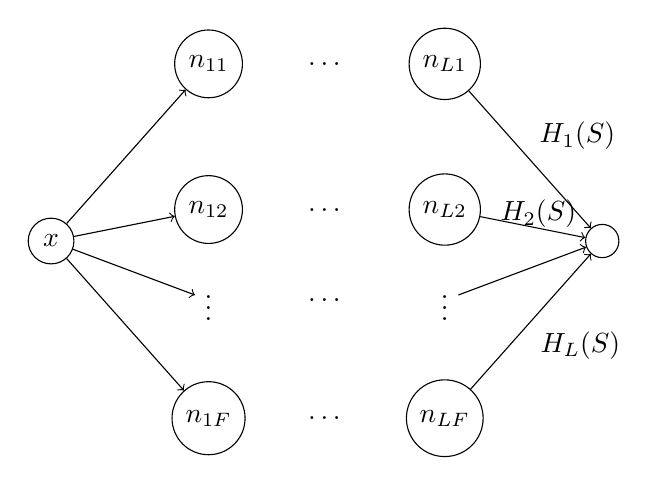
\begin{tikzpicture}
                \node[draw,circle] (x) at (0,0) {$x$};
                
                \node[draw,circle] (n11) at (2 ,2.25) {$n_{11}$};
                \node[draw,circle] (n12) at (2 ,0.4) {$n_{12}$};
                \node (vdot1) at (2 ,-0.75) {$\vdots$};
                \node[draw,circle] (n1F) at (2,-2.25) {$n_{1F}$};
                
                \node at (3.5 ,2.25) {$\dots$};
                \node at (3.5 ,0.4) {$\dots$};
                \node at (3.5 ,-0.75) {$\dots$};
                \node at (3.5 ,-2.25) {$\dots$};
                
                \node[draw,circle] (nL1) at (5 ,2.25) {$n_{L1}$};
                \node[draw,circle] (nL2) at (5 ,0.4) {$n_{L2}$};
                \node (vdot2) at (5 ,-0.75) {$\vdots$};
                \node[draw,circle] (nLF) at (5,-2.25) {$n_{LF}$};
                

                \node[draw,circle] (out) at (7,0) {$\ $};

                \path[draw,->] (x) -- (n11);
                \path[draw,->] (x) -- (n12);
                \path[draw,->] (x) -- (vdot1);
                \path[draw,->] (x) -- (n1F);

                \path[draw,->] (nL1) -- node[midway,above right] {$H_{1}(S)$} (out);
                \path[draw,->] (nL2) -- node[near start,above right=-0.2cm] {$H_{2}(S)$} (out);
                \path[draw,->] (vdot2) -- (out);
                \path[draw,->] (nLF) -- node[midway,below right] {$H_{L}(S)$} (out);

            \end{tikzpicture}
            \caption{Shape of $\Phi$.}
            \label{fig:shape_phi}
        \end{figure}

            By definition of $\Phi$, we can then write:

            $$ \Phi(S,x) =  \sigma \left( \Sum{i=1}{F_L} H_i(S) \Phi^{(L)}_i(S,x) \right) .$$

            As a consequence we have the inequalities:
            \begin{align*}
                ||\Phi(S,x)|| &\leq \Sum{i=1}{F_L} ||H_i(S) \Phi^{(L)}_i(S,x) || \\
                &\leq F_L \ninf{H^{(L)}} || \Phi^{(L)}_i(S,x) || \\
                &\leq F_L \ninf{H^{(L)}} \left( \Prod{i=0}{L-1} F_i \right) \left( \Prod{i=0}{L-1} \ninf{H^{(i)}} \right) ||x|| \\
                &= \left( \Prod{i=0}{L} F_i \right) \left( \Prod{i=0}{L-1} \ninf{H^{(i)}} \right) ||x||
            \end{align*}

            where we used the induction hypothesis to bound $|| \Phi^{(L)}_i(S,x) ||$. This concludes the proof of the lemma.\\
        
            We now prove theorem \ref{thm:stability_general} by induction on the number of layers $L$ as well.
            Firstly, if we consider a GNN with 1 layer, then $\Phi(S,x)$ is $\sigma(H(S)x)$ with $H(S) = aS + b I_N$. Given two symmetric matrices $S$ and $\hat{S}$ and a vector $x \in \mathbb{R}^N$, the theorem is written:
                $|| \sigma(H(S)x) - \sigma(H(\hat{S})x) || \leq B_1 \op{S - \hat{S}} ||x||$ with $B_1 = A^{(1)} = |a|$.

                This holds since:
                \begin{align*}
                    || \sigma(H(S)x) - \sigma(H(\hat{S})x) || &\leq || H(S)x - H(\hat{S})x || \\
                    &= || a (S - \hat{S}) x|| \\
                    &\leq |a| \op{S - \hat{S}} ||x||.
                \end{align*}
            
            We now consider $L \in \mathbb{N}^*$ and we assume that the theorem is true for all GNNs with $L$ layers satisfying the hypotheses. I.e., if $\Psi$ is such a GNN, $|| \Psi (S,x) - \Psi (\hat{S},x) || \leq B_L \op{S - \hat{S}} ||x||.$

            We consider a GNN $\Phi$ with $L+1$ layers and use the exact same notations as in the proof of the lemma.


            We begin by bounding $\Phi(S,x) - \Phi(\hat{S},x)$ with the $\Phi^{(L)}_i$:
            \begin{align}
                || \Phi (S,x) - \Phi (\hat{S},x) || &= || \Sum{i=1}{F_L} \ H_i (S) \sigma(\Phi^{(L)}_i (S,x)) - H_i (\hat{S}) \sigma (\Phi^{(L)}_i (\hat{S},x)) \ || \nonumber \\
                &\leq \Sum{i=1}{F_L} || H_i (S) \sigma(\Phi^{(L)}_i (S,x)) - H_i (\hat{S}) \sigma (\Phi^{(L)}_i (\hat{S},x)) \ || \nonumber \\
                &\leq \Sum{i=1}{F_L}  || H_i (S) \left(\sigma(\Phi^{(L)}_i (S,x)) - \sigma (\Phi^{(L)}_i (\hat{S},x)) \right) || \nonumber \\
                &+  \Sum{i=1}{F_L} || \ (H_i(S) - H_i(\hat{S}) ) \sigma (\Phi^{(L)}_i (\hat{S},x)) \ || 
                \label{eq:bound_phi_raw}
            \end{align}

            We should now bound both terms separately. We begin with $|| H_i (S) \left(\sigma(\Phi^{(L)}_i (S,x)) - \sigma (\Phi^{(L)}_i (\hat{S},x)) \right) ||$. Using the definition of $\ninf{H^{(L)}}$ and the induction hypothesis, we get:
            \begin{align}
                || H_i (S) &\left(\sigma(\Phi^{(L)}_i (S,x)) - \sigma (\Phi^{(L)}_i (\hat{S},x)) \right) || \\ 
                &\leq \ninf{H^{(L)}} || \sigma(\Phi^{(L)}_i (S,x)) - \sigma (\Phi^{(L)}_i (\hat{S},x))|| \nonumber \\
                &\leq \ninf{H^{(L)}} || \Phi^{(L)}_i (S,x) - \Phi^{(L)}_i (\hat{S},x)|| \nonumber \\
                &\leq \ninf{H^{(L)}} B_L \op{S - \hat{S}} ||x||.\label{eq:bound_first_term}
            \end{align}

            For the second term, using the definition of $A^{(L)}$ and the lemma, we get:
            \begin{align}
                || (H_i(S) - H_i(\hat{S}) ) & \sigma (\Phi^{(L)}_i (\hat{S},x)) || \nonumber \\
                &\leq \op{H_i(S) - H_i(\hat{S})} ||\sigma (\Phi^{(L)}_i (\hat{S},x)) || \nonumber \\
                &\leq A^{(L)} \op{S-\hat{S}} ||\Phi^{(L)}_i (\hat{S},x)|| \nonumber \\
                &\leq A^{(L)} \op{S-\hat{S}} \left( \Prod{i=0}{L-1} F_i \right) \left( \Prod{i=0}{L-1} \ninf{H^{(i)}} \right) ||x||\label{eq:bound_second_term}.
            \end{align}


            Combining the bounds given by inequalities \ref{eq:bound_first_term} and \ref{eq:bound_second_term} in the inequality \ref{eq:bound_phi_raw} yields

            \begin{align}
                || \Phi (S,x) - \Phi (\hat{S},x) || &\leq \Sum{i=1}{F_L}  \ninf{H^{(L)}} B_L \op{S - \hat{S}} ||x|| \nonumber \\
                &+ \Sum{i=1}{F_L} A^{(L)} \left( \Prod{i=0}{L-1} F_i \right) \left( \Prod{i=0}{L-1} \ninf{H^{(i)}} \right) \op{S-\hat{S}} ||x|| \\
                & \leq \left( F_L \ninf{H^{(L)}} B_L + F_L A^{(L)} \left( \Prod{i=0}{L-1} F_i \right) \left( \Prod{i=0}{L-1} \ninf{H^{(i)}} \right) \right) \op{S-\hat{S}} ||x||.
            \end{align}

            Given that $F_L \ninf{H^{(L)}} B_L + F_L A^{(L)} \left( \Prod{i=0}{L-1} F_i \right) \left( \Prod{i=0}{L-1} \ninf{H^{(i)}} \right) = B_{L+1}$, this can be rewritten:

            \begin{equation}
                || \Phi (S,x) - \Phi (\hat{S},x) || \leq B_{L+1} \op{S - \hat{S}} ||x||,
            \end{equation}

            which shows that the theorem holds for GNN with $L+1$ layers and concludes the proof.

        \end{proof}



   \subsection{Node embedding stability}

    In this section, we discuss two corollaries of the theorem \ref{thm:stability_general} that translate the original result in two stability properties at the node embedding level. Like for the theorem, in the bounds we can replace $L A (F \ninf{H})^{L-1} $ by $B_L$. 
    
    The node embeddings are defined in section \ref{TODO:define node embedings}.

    \begin{corollary}
    \label{cor:k-hop_node_stability}
    We consider a GNN $\Phi$ satisfying the hypotheses of theorem \ref{thm:stability_general}, and a couple of graph $G,\hat{S}$ with their associated shift operators $S,\hat{S}$. We assume that all the columns of the initialisation matrices $X^{(0)}$ are normalized. If we consider the $i$-th nodes of $G$ and $\hat{G}$, noted $v_i$ and $v'_i$ and assume that their $k$-hop are equal, then we have the following property:
    
    \begin{align}
        || \Phi(S, X^{(0)})_{v_i} &- \Phi(\hat{S}, X ^{(0)}_{v'_i}|| \nonumber \\
        &\leq \sqrt{d} B_L^{(k)} \op{S - \hat{S}}
        \label{eq:k-hop_node_stab}
    \end{align}

    where we define $$ B_L^{(k)} = \left( \Prod{i=1}{L-1} F_i \right)  \cdot \Sum{i=k+1}{L} \left[ (\underset{j=L-i+1}{\overset{L-1}{\prod}} \ninf{H ^{(i)}}) \cdot A^{(L-i)} \cdot (\underset{j=0}{\overset{L-i-1}{\prod}} \ninf{H ^{(i)}}) \right].$$ 

    We can bound $B_L^{(k)}$ is $0$ if $L \geq k$ and it can be bounded by $(L-k) A (F \ninf{H})^{L-1}$ otherwise.

    \end{corollary}

     The hypothesis of normalization is not necessary, it is there so the statement is more readable. Noting $C_i$ the columns of $X$, we could remove the hypothesis and replace $\sqrt{d}$ by $\sqrt{\Sum{i=1}{d} || C_i||^2 }$.


    \begin{corollary}
    \label{cor:global_node_stability}
    We consider a GNN $\Phi$ satisfying the hypotheses of theorem \ref{thm:stability_general}, and a couple of graph $G,\hat{S}$ with their associated shift operators $S,\hat{S}$. We assume that all the columns of the initialisation matrices $X^{(0)}$ are normalized. We can control the total squared distances between the embeddings:
    
    \begin{equation}
        \Sum{i=1}{N} || \Phi(S, X^{(0)})_{v_i} - \Phi(\hat{S}, X ^{(0)})_{v'_i} ||^2 \leq d M^2
        \label{eq:global_node_stab}
    \end{equation}

    where $M$ is a bound of theorem \ref{thm:stability_general}, i.e. $ M = L A (F \ninf{H})^{L-1} \op{S - \hat{S}}$ or $M=B_L \op{S - \hat{S}}$.

    \end{corollary}

        This last property is interesting because it ensures that for most nodes $ || \Phi(S, X^{(0)})_{v_i} - \Phi(\hat{S}, X ^{(0)})_{v'_i} ||^2 \leq \frac{\sqrt{d} M}{\sqrt{N}}$. Since the bound $d M^2$ does not depend on $N$, this means that using a GNN with fixed parameters on large database gives reliable embeddings for the majority.

        The worst case distance for two embeddings can still be relatively large, it is bounded by 
        \begin{align*}
            || \Phi(S, X^{(0)})_{v_i} - \Phi(\hat{S}, &X ^{(0)})_{v'_i} || \\
            &\leq \sqrt{\Sum{i=1}{N} || \Phi(S, X^{(0)})_{v_i} - \Phi(\hat{S}, X ^{(0)})_{v'_i} ||^2} \\
            &\leq \sqrt{d}M,
        \end{align*} 

        but this cannot happen for several nodes at the same time.

        \begin{proof}
            We prove the corollary \ref{cor:global_node_stability}. We consider $\Phi$, $S$, $\hat{S}$ and $X^{(0)}$ as in the statement of the corollary.

            By definition of the embedding, $|| \Phi(S, X^{(0)})_{v_i} - \Phi(\hat{S}, X ^{(0)})_{v'_i} || = || L_i || ^2$ where $L_i$ is the $i$-th line of the matrix $\Phi(S,X^{(0)}) - \Phi(\hat{S},X^{(0)})$. Therefore, 
            \begin{align*}
                \Sum{i=1}{N} || \Phi(S, X^{(0)})_{v_i} - \Phi(\hat{S}, X ^{(0)})_{v'_i} ||^2 &= \Sum{i=1}{N} || L_i ||^2 \\
                &= \Sum{j=1}{d} || C_j ||^2 \\
                &= \Sum{j=1}{d} || \Phi(S,C^{(0)}_j) - \Phi(\hat{S},C^{(0)}_j) ||^2 
            \end{align*}

            where $C_j$ is the $j$-th column of the matrix $\Phi(S,X^{(0)}) - \Phi(\hat{S},X^{(0)})$ and $C^{(0)}_j$ is the $j$-th column of $X^{(0)}$.

            Since theorem \ref{thm:stability_general} ensures that $ || \Phi(S,C^{(0)}_j) - \Phi(\hat{S},C^{(0)}_j) || \leq M $, we deduce:
            $$ \Sum{i=1}{N} || \Phi(S, X^{(0)})_{v_i} - \Phi(\hat{S}, X ^{(0)})_{v'_i} ||^2 \leq d M^2. $$

        \end{proof}

    \subsection{Instantiation for Databases}
     
    \begin{definition}{Error relative to the perturbation}
        Let $\mathbb{D}_1$ and $ \mathbb{D}_2 = \pi(\mathbb{D}_1)$ be a database and a perturbed database generated from $\mathbb{D}_1$. We define the error relative to the perturbation as $\varepsilon =  \op{ S_{\Gamma(\mathbb{D}_1)} - S_{\Gamma(\mathbb{D}_2)} }$, where the matrix $S_{\Gamma(\mathbb{D}_2)}$ is built such that the rows and columns that represent an element of $\mathbb{D}_2$ corresponds to the rows and columns of its original counterpart in $\mathbb{D}_1$.
    \end{definition}


    \begin{corollary}
    
    We consider a GNN $\Phi$ satisfying the hypotheses of theorem \ref{thm:stability_general}, a database $\mathbb{D}_1$ with a perturbed database $\mathbb{D}_2$ and a node $v$ in $\Gamma(\mathbb{D}_1)$ that is identified to the node $v'$ in  $\Gamma(\mathbb{D}_2)$. Assuming that all the columns of the initialisation matrices $X^{(0)}$ are normalized, we have the following property:
    
    \begin{align}
        || \Phi(S_{\Gamma(\mathbb{D}_1)}, X^{(0)})_v - \Phi(P_0^T &S_{\Gamma(\mathbb{D}_2)} P_0, P_0^T \hat{X}^{(0)})_{v'}|| \\
        &\leq \sqrt{d} B_L \op{S_{\Gamma(\mathbb{D}_1)} - S_{\Gamma(\mathbb{D}_2})} ||x||)
    \end{align}

    In equation \ref{eq:node_stab},  $v$ and $v'$ being identified means that they represent the same row in $S_{\Gamma (\mathbb{D}_1)}$ and $S_{\Gamma(\mathbb{D}_2)}$ respectively. 
    \end{corollary}

\begin{definition}[Downstream tasks stability (fig: \ref{fig:stability})]
    The DST stability translate the capacity of two embeddings of the same element or value, generated from the perturbed and the clean databases, to gives the same result when they are used as input for downstream tasks.\\

    This is schematised by the last line of the figure, \ref{fig:stability}. In the last line of the figure, are compared the results of downs stream tasks computed from $\mathbb{D}$ and the ones obtained using $\pi (\mathbb{D})$. In this figure, we are not comparing from which embedding we are retrieving the highest accuracy, but if the results obtained from the two structures are similar. 
\end{definition}

	\bibliographystyleGnn{apalike}
	\bibliographyGnn{biblio_gnn}

\end{document}